\documentclass[12pt,letterpaper]{article}
\usepackage{listings,lstautogobble}
\usepackage[usenames,dvipsnames]{xcolor}
\usepackage{framed}
\usepackage{xcolor}
\usepackage{pgfornament}
\usepackage{graphicx}
\renewcommand{\familydefault}{\sfdefault}
\definecolor{light-gray}{gray}{0.95}
\lstdefinelanguage{budget}{
    autogobble=true,
    basicstyle=\color{ForestGreen}\ttfamily\small,
    keywordstyle=[0]\color{black}\bf,
    keywordstyle=[1]\color{NavyBlue},
    keywordstyle=[2]\color{RoyalBlue},
    keywords=[0]{budget,.budget_conf},
    keywords=[1]{summary, detail, import, help, sum, det, imp, h, su},
    keywords=[2]{transactions, categories, category, period, month, year, y, sortby, trans, cat, per, mo, c, s, M},
}
\lstnewenvironment{budget}[1][]
{
    \lstset{language={},
    autogobble=true,
    linewidth=4.5in,
    backgroundcolor=\color{light-gray},
    basicstyle=\color{ForestGreen}\ttfamily\small,
    keywordstyle=[0]\color{black}\bf,
    keywordstyle=[1]\color{NavyBlue},
    keywordstyle=[2]\color{RoyalBlue},
    keywords=[0]{budget},
    keywords=[1]{summary, detail, import, help, sum, det, imp, h, su},
    keywords=[2]{transactions, categories, category, period, month, year, y, sortby, trans, cat, per, mo, c, s, M},
#1}}{\vspace{0.2in}}    
\newcommand{\eachpageornament}{%
    \begin{tikzpicture}[remember picture, overlay]
        \node[anchor=north west] at (current page.north west){%
            \pgfornament[width=2cm]{63}};
            \node[anchor=north east] at (current page.north east){%
                \pgfornament[width=2cm,symmetry=v]{63}};
                \node[anchor=south west] at (current page.south west){%
                    \pgfornament[width=2cm,symmetry=h]{63}};
                    \node[anchor=south east] at (current page.south east){%

\pgfornament[width=2cm,symmetry=c]{63}};
                    \end{tikzpicture}
                }
\begin{document}
\begin{framed}
    \begin{minipage}[t][3in][t]{5in}
        \resizebox{5in}{3in}{%
            \begin{tikzpicture}[rotate=90, transform shape]
                \node[inner sep=0pt] 
                {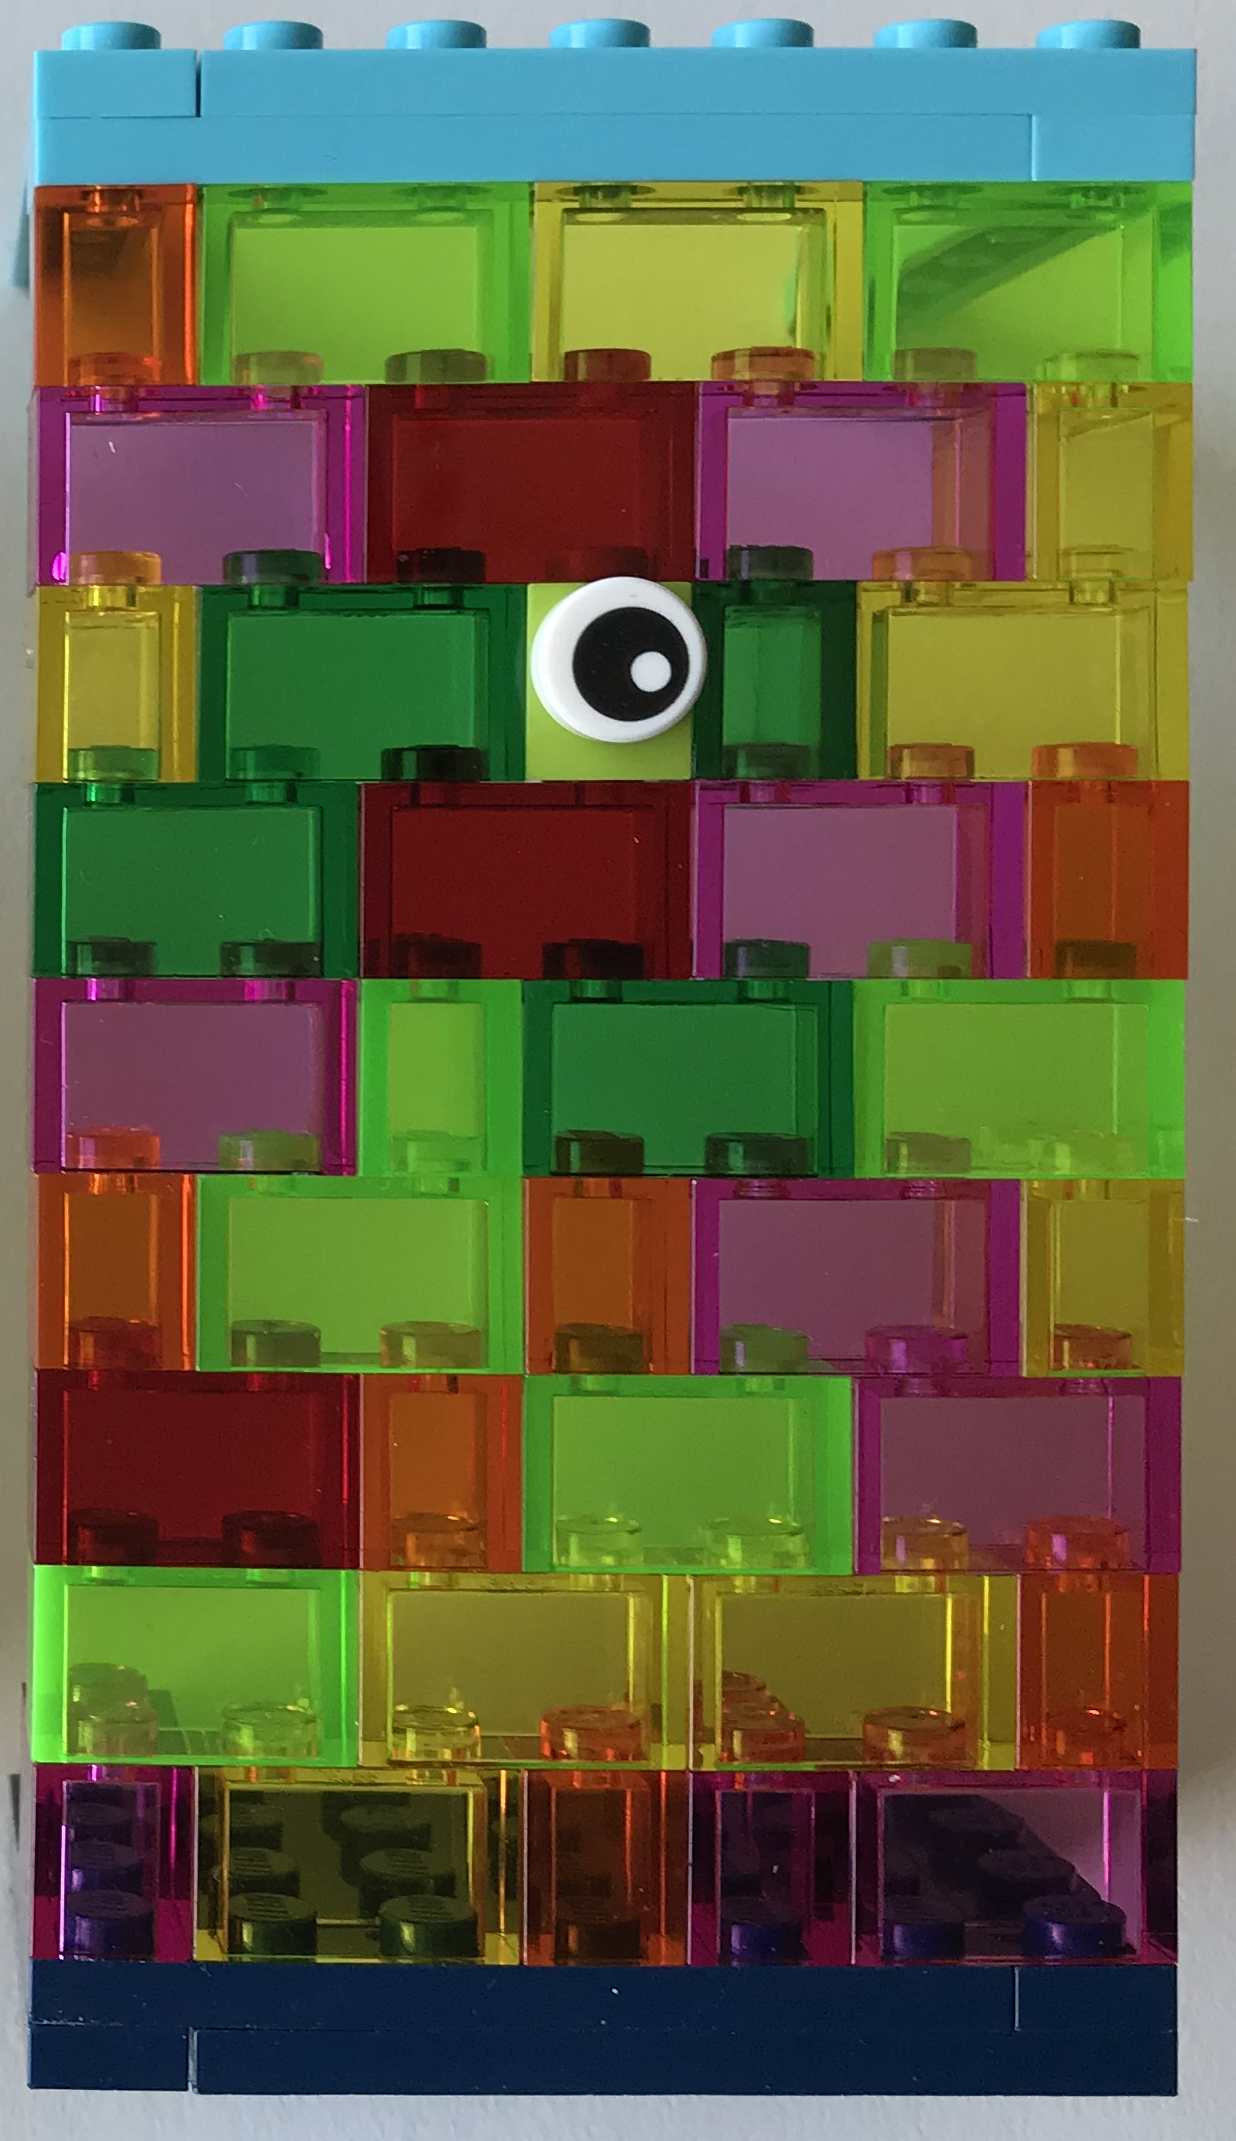
\includegraphics[width=.25\textwidth]{LegoTDD.png}};
            \end{tikzpicture}
        }
\end{minipage}
\end{framed}
\Large
\begin{framed}
    \begin{minipage}[t][3in][t]{5in}
        You can abbreviate every command and option! \\ \\
        the command:
        \begin{budget}
            budget detail category Groceries sortby M
        \end{budget}
        is equivalent to: 
        \begin{budget}
            budget det cat Groceries sor M
        \end{budget}
        is equivalent to: 
        \begin{budget}
            budget d c Groceries s M
        \end{budget}
    \end{minipage}
\end{framed}
\begin{framed}
    \begin{minipage}[t][3in][t]{5in}
        You can have a summary of your favorite categories 
        \large
        \begin{enumerate}
            \item write your categories in a CSV file
                \begin{itemize}
                    \item one category per line
                    \item no quotes
                \end{itemize}
                \begin{budget}
                    Groceries
                    Business Expenses
                    Credit Card Payments
                \end{budget}
            \item use the \lstinline[language=budget,basicstyle=\large]!categories! options:
                \begin{budget}
                    budget summary categories MyFavorite.csv 
                \end{budget}
        \end{enumerate}
    \end{minipage}
\end{framed}
\begin{framed}
    \begin{minipage}[t][3in][t]{5in}
        \large
        You can show the detail of any transaction file\\ \\
        use the \lstinline[language=budget,basicstyle=\large]!transactions! options: \\
        \begin{budget}
            budget detail transactions Download202003.csv
        \end{budget}
    \end{minipage}
\end{framed}
\begin{framed}
    \begin{minipage}[t][3in][t]{5in}
        \Large
        You can select data for a given period of time\\

        use the \lstinline[language=budget,basicstyle=\Large]!period! option followed by two dates
        \begin{itemize}
            \item dates should be in the format \texttt{MM/DD/YYYY}
            \item in which order doesn't matter
        \end{itemize}
        \begin{budget}
            budget detail period 01/01/2020 01/31/2020

            budget summary p 10/17/2020 01/23/2020 
        \end{budget}
    \end{minipage}
\end{framed}
\begin{framed}
    \begin{minipage}[t][3in][t]{5in}
        \Large
        You can select data for a given month or year

        use \lstinline[language=budget,basicstyle=\large]!month! then the year and month\\
        \begin{budget}
            budget summary month 2020 03

            budget detail mo 2020 12
        \end{budget}
        use  \lstinline[language=budget,basicstyle=\large]!year! then the year\\
        \begin{budget}
            budget summary year 2020

            budget detail y 2020
        \end{budget}
    \end{minipage}
\end{framed}
\begin{framed}
    \begin{minipage}[t][3in][t]{5in}
        \Large
        You can sort transactions with several criteria\\

        use the \lstinline[language=budget,basicstyle=\Large]!sortby! option followed by letters
        \begin{itemize}
            \item \textbf{D} for date, \textbf{M} for amount, \textbf{C} for category
            \item \textbf{N} for name, \textbf{A} for account, \textbf{O} for note
            \item uppercase letter means ascending order
            \item lowercase letter means descending order
        \end{itemize}
        \begin{budget}
            budget detail sortby CDm
        \end{budget}
    \end{minipage}
\end{framed}
\begin{framed}
    \begin{minipage}[t][3in][t]{5in}
        \Large
        You can sort the summary by category or amount\\

        use the \lstinline[language=budget,basicstyle=\Large]!sortby! option followed by letters
        \begin{itemize}
            \item \textbf{C} for category
            \item \textbf{M} for amount
            \item uppercase letter means ascending order
            \item lowercase letter means descending order
        \end{itemize}
        \begin{budget}
            budget summary sortby m
        \end{budget}
    \end{minipage}
\end{framed}
\begin{framed}
    \begin{minipage}[t][3in][t]{5in}
        \Large
        The rules for importing transactions:\\
        \normalsize
        \begin{minipage}[t]{4in}
            \begin{itemize}
                \item files containing transactions that are already imported are rejected
                \item a transaction is already imported if there is already a transaction with the same date, name, and amount in the main transaction file 
                \item transactions with a status different from \emph{posted} are not imported 
                \item transactions with a status \emph{posted} are imported and this info is replaced with the account name
                \item transactions where the account name is already set are imported, but their account name is unchanged.
            \end{itemize}
        \end{minipage}

    \end{minipage}
\end{framed}
\begin{framed}
    \begin{minipage}[t][3in][t]{5in}
        \Large
        You can import a file and set the account name\\
        \begin{budget}
            budget import Download.csv "Checkings"
        \end{budget}
        Or you can omit the account name
        \begin{itemize}
            \item the account name is \emph{in } the file name
            \item exclusive of the digits
        \end{itemize}
        \begin{budget}
            budget import "Checkings202003.csv"
        \end{budget}
    \end{minipage}
\end{framed}
\begin{framed}
    \begin{minipage}[t][3in][t]{5in}
        \Large
        You can import a whole directory \\
        \normalsize
        \begin{budget}
            ls data/Downloads 
            BusinessChecking202003.csv
            BusinessSparkVisa202003.csv
            ChasePersonalCredit202003.csv
            JointChecking202003.csv
            JointSaving202003.csv
            PersonalChecking202003.csv
            PersonalSavings202003.csv
        \end{budget}
        all the files will be imported\\
        the account name will depend on each file name. 
        \begin{budget}
            budget import data/Downloads
        \end{budget}
    \end{minipage}
\end{framed}
\begin{framed}
    \begin{minipage}[t][3in][t]{5in}
        \Large
        Where is your main transactions files?\\ \\
        Look into the file \lstinline[language=budget,basicstyle=\Large]!.budget_conf! in your home directory 
        \normalsize
        \begin{budget}
            cat ~/.budget_conf
            TRANSACTIONS:/Users/you/data/Transactions.csv
        \end{budget}
        \Large
        Or better, use the \lstinline[language=budget,basicstyle=\Large]!help! command.
        \begin{budget}
            budget help configuration 
            TRANSACTIONS:/Users/you/data/Transactions.csv
        \end{budget}
    \end{minipage}
\end{framed}
\begin{framed}
    \begin{minipage}[t][3in][t]{5in}
        \Large
        What is the transaction file CSV format?\\
        \normalsize
        \begin{enumerate}
            \item account (in download files: status)
            \item unused
            \item date (DD/MM/YYYY)
            \item notes
            \item name
            \item category
            \item amount
        \end{enumerate}
    \end{minipage}
\end{framed}
\end{document}
